\myPhantom{paragraph}{Conclusion générale}
Nous avons développé une plateforme open source, permettant le prototypage rapide d'activités \tiret{d'enseignement ou de recherche} en robotique. Le dispositif Poppy Éducation, à travers le kit ErgoJr, a connu un retour plutôt positif de la part de la communauté scolaire.
L'équipe Poppy Éducation a pu observer ces retours et les pratiques qui y ont mené, et cela tant qualitativement que quantitativement. Qualitativement, les enseignants en témoignent:
\citeAtion{GLassus}
%Le robot ErgoJr est arrivé au lycée l’année dernière (2016). Je n’avais jamais enseigné la robotique auparavant et le fait de commencer le projet avec 8 robots (et les contraintes matérielles que cela puisse impliquer) était intimidant. Au final, le kit pédagogique a été très bien accueilli par les élèves en option ICN et le corps enseignant. Il est même devenu un élément incontournable de mon enseignement de l’informatique. De plus, Snap! a complètement changé mon approche de l’apprentissage de l’algorithmique.
Ce kit a même parfois dépassé nos espérances \tiret{qualitatives} en impactant considérablement certains comportements, chez les élèves, mais aussi chez les enseignants; c'est notamment ce que relate cet autre enseignant:
\citeAtion{LVincent}
%J’avais déjà deux robots à disposition dans ma salle de cours et quand Inria nous a prêté 10 ErgoJr, nous avons constitué 10 groupes de 2 élèves. Cela me permet de travailler sur des thèmes différents et de créer des projets qui passionnent les élèves. Ces robots sont si fascinants que des élèves qui ne sont pas en 2nd ICN viennent même assister aux cours en tant qu’invités ! J’ai pu aussi enrichir mes compétences en programmation avec Snap! et Python grâce à Poppy Education.
Le kit pédagogique ErgoJr a été co-conçu par des enseignants des sections \sht{ICN} et \sht{ISN} (nouvelles à cette époque), mais il hérite de nombreuses caractéristiques issues de sa plateforme mère: Poppy. Celle-ci a également fait ses preuves (qualitatives) dans d'autres niveaux de l'éducation, comme dans l'enseignement supérieur avec, par exemple, le robot Torso:
\citeAtion{JLCharles}
%Cela fait deux ans que j’utilise Poppy Torso dans mes cours. Il permet de relever des défis d’enseignement pour donner envie aux élèves d’apprendre la conception, le design, la CAO, la mécanique, la programmation, les matériaux; toutes ces matières sont beaucoup plus difficiles à enseigner avec les anciennes méthodes. Les élèves deviennent acteurs et moteurs de leur cursus. Le fait qu’il y ait une plateforme matérielle à partager avec l’enseignant et les élèves, c’est un point de rencontre pédagogique, et ça, ça donne une force très importante à la pédagogie par projets.
De nouveaux enseignants souhaitant utiliser le kit ErgoJr ont été identifiés, cela nous permettra d'effectuer de nouvelles passations des questionnaires présentés ici et ainsi de comparer les résultats à plus large échelle;
car, les enseignants ayant participé à la phase d'évaluation ont également participé à la phase de conception, et sont tous de la région Nouvelle Aquitaine, il est donc difficile de généraliser.
À noter également qu'il faut distinguer les effets induits par \gui{les nouvelles technologies} et \gui{les sciences du numérique}: Les ordinateurs installés dans les établissements scolaires dans les années 1990 ne produisent plus le même attrait chez les étudiants.
Multiplier les essais pour limiter l'effet de nouveauté et élargir la zone géographique, représentent la prochaine étape vers la généralisation de nos résultats.\par%
Mais, une conclusion majeure pouvant déjà être tirée est qu'il est inutile de fournir un matériel ne fonctionnant que pour les usages qui ont été prescrits pour lui; il faut un matériel souple et robuste s'adaptant aux besoins (fluctuants) des utilisateurs en offrant une utilisabilité suffisante pour permettre une appropriation rapide. 
\begin{figure}[!h]
    \begin{minipage}{0.5\linewidth}
        \centering
        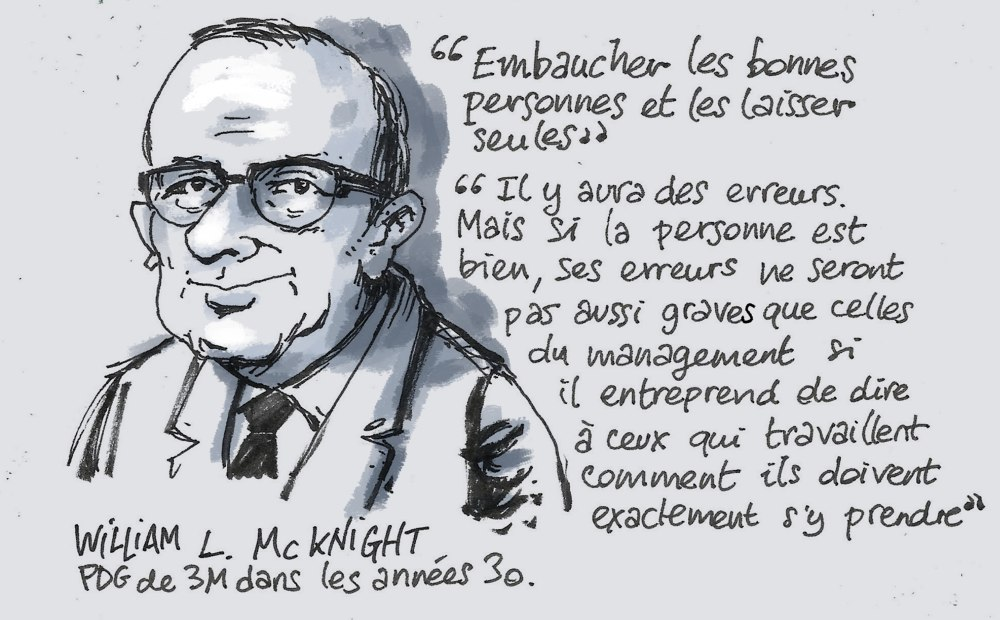
\includegraphics[width=\linewidth]{Figures/Duriez-motiv5.jpg}
        \caption[W, L.MacKnight, citation]{W, L.MacKnight, \textit{ill.} F.~Duriez~\citeURL{motiv_pic}}
        \label{fig:motiv5}
    \end{minipage}
    \hfill
    \begin{minipage}{0.475\linewidth}
    \myDefautStyle
        Pour bien faire, il faut donc laisser l'enseignant libre, et comme le dit William L.MacKnight, il y aura des erreurs, mais moins graves que si elles émanaient des prescripteurs (ici, l'État au travers des programmes officiels ou les développeurs de technologies) plutôt que des individus sur le terrain (ici, les enseignants).\\
    \end{minipage}
\end{figure}\par%
Pour cela, nous venons de voir que la plateforme Poppy, notamment le robot ErgoJr, pouvait avoir une grande variété d'usages et que ceux-ci affectaient significativement la perception qu'ont les utilisateurs de la robotique; du moins, qu'ils affectaient les réponses au questionnaire \sht{EURO382}.
Cependant, certains éléments du kit \tiret{atouts comme faiblesses} ne font pas l'unanimité chez les utilisateurs. Dresser une carte d'identité du kit ErgoJr, notamment en matière d'utilisabilité (\cf \sht{SUS}) et d'\sht{UX} (\cf \sht{ATT}), puis la comparer à d'autres kits, comme ici, avec le kit Inirobot (\ie robot Thymio) permet de contribuer à une meilleure visibilité des différents dispositifs proposés aux enseignants dans le cadre de l'apprentissage des sciences du numérique, en ne se limitant pas à ses caractéristiques techniques.\par%
Dans ce même objectif a été mis en place un protocole de suivi de cohorte qui devait être activé à la rentrée de septembre 2017. Ce protocole devait nous permettre une analyse longitudinale et écologique afin d'observer l'impact de ce kit robotique dans les apprentissages et les représentations qu'ont les élèves de la pensée informatique. Celui-ci n'a pas pu être déployé comme convenu. Mais d'autres résultats issus de passations ponctuelles ont permis de quantifier l'impact de différents aspects de ces ressources sur des dimensions de motivation, d'acceptabilité (de la robotique) ou de connaissances.\par%
En effet, nous avons vu qu'une chose aussi banale que de nommer un objet, ici un robot Poppy Humanoïde, affectait positivement notre perception de celui ci (au sens de notre capacité à reconnaître des émotions qu'il mimait); mais, que cette action amplifiait notre \cro{peur} plus globale pour la robotique (\cf \sht{NARS}). Mais, il convient de préciser, que même si cela l'amplifiait, le niveau de \cro{peur} (score au \sht{NARS}) avant l'observation du robot est toujours plus élevé, quelles que soient les conditions, relevant d'une certaine accommodation à cette technologie pendant l'observation (se traduisant par un score plus faible au \sht{NARS}).\par%
Concernant la motivation un phénomène inattendu a été observé. En effet, entre deux tâches où, objectivement, l'une offrait plus de contrôle à l'élève, nous avons relevé \tiret{grâce au questionnaire \sht{IMI}} que la perception du contrôle de l'activité a été plus faible dans cette condition. Pour interpréter ce résultat, nous nous sommes appuyés sur nos observations qui étaient que dans ce groupe le contrôle accru a permis l'émergence d’un leadership au sein des individus des minis groupes constitués, rendant le sentiment de contrôle pour les autres membres du groupe plus faible. Mais d'autres études sont nécessaires afin de préciser ces résultats.\par%
D'autres résultats qualitatifs sont venus confirmer nos premières hypothèses, comme la plus value à exploiter la manipulation sur ces objets tangibles ici présentés dans deux contextes: l'un portant sur la possibilité d'exploiter uniquement une version simulée (perdant l'aspect tangible de l'outil); l'autre, illustrant deux possibilités de rédaction de \sht{TD} (l'une exploitant davantage l'aspect tangible que l'autre). Dans ces deux cas, l'aspect tangible a été un plus, tant qualitativement que quantitativement. Et ceci, que ce soit d'un point de vue motivationnel que d'un point de vue d'appréhension des concepts abordés.\par%
De plus, ces évaluations permettent de poser les fondations d'études plus complexes, notamment sur les apprentissages réalisés par les élèves, leur motivation et leur engagement dans les activités, l'évolution de leur perception des robots, de l'intelligence artificielle, et plus généralement leur appropriation de la pensée informatique.\par%
L'ensemble des ressources pédagogiques constituées représente en soit une réussite du projet qu'il reste à pérenniser notamment en intégrant ces résultats.
%Enfin, d'autres résultats restent à analyser ou compléter, il est difficile d’aller plus loin aujourd'hui dans leur interprétation sans de nouvelles données comme par exemple avec le score obtenu au SUS par les enseignants ($0,57$) plus faible que celui traditionnellement relevé ($0,72$).